
\chapter{The Large Hadron Collider and the ATLAS Detector}
\label{ch:lhc_atlas_detector}

The Large Hadron Collider (LHC)~\cite{LHCMachine,LHC1,LHC2, LHC3} is a synchrotron collider located at the Conseil Européen pour la Recherche Nucléaire (CERN) near Geneva, Switzerland.
It is also the world's most powerful particle accelerator, providing both proton-proton ($pp$) and heavy ion collisions at the high energy frontier.
At maximum speed, the protons in the LHC are only $3~\mps$ slower than the speed of light.

Four primary experiments utilize the $\TeV$ scale collisions generated the each of the the four interaction points (IPs) of the LHC.
Two general-purpose experiments, ATLAS~\cite{ATLAS} and CMS~\cite{CMS}, employ hermetic detectors to study various physics processes.
The LHCb experiment~\cite{LHCb} focuses on measuring the properties of B mesons and other particles containing b-quarks, which are significant for understanding CP violation.
The Alice experiment~\cite{ALICE} investigates the properties of quark-gluon plasma, a state of matter believed to have existed in the early universe.
Additionally, the LHC hosts several smaller, highly specialized experiments including LHCf~\cite{LHCf}, TOTEM~\cite{TOTEM}, MoEDAL~\cite{MoEDAL}, FASER~\cite{FASER}, and SND@LHC~\cite{SNDLHC}.
All LHC experiments strive to answer fundamental questions about the universe; to test the predictions of the Standard Model of particle physics or to search for new physics beyond it.

This section describes common collider physics definitions, such as the coordinate system and luminosity,
the LHC along with its injector chain, and the ATLAS experiment.
As the focus of this work is on data and tools for $pp$ collisions at the LHC, the discussion is limited to this context.

\section{The Large Hadron Collider}

The LHC is a somewhat circular collider with a circumference of $26.7~\km$.
It is closer to an irregular octagon with rounded corners and approximately $ 530~\m $ long straight sections, housed within a tunnel whose depth varies between $45~\m$ and $170~\m$ underground.

The machine consists of two ring acceleration pipes, each carrying a separate beam of protons or heavy ions that are accelerated in opposite directions.
The beams are surrounded by 1232 superconducting NbTi dipole magnets that generate an $8.33~\tesla$ magnetic field to bend the protons around the curved sections of the ring.
Many more higher-order multipole magnets are used for beam insertion, cleaning, dumping, and focusing towards the experiment IPs.
Along one of the straight sections, 16 superconducting radiofrequency cavities, eight per beam, operate at $400~\MHz$ to accelerate the protons to their maximum energy.
The LHC was designed to deliver a centre-of-mass energy of $\sqrt{s}=14~\TeV$ but has yet to reach this due to technical limitations.

The beams are not continuous streams of protons but are instead segmented into bunches, each containing on the order of $10^{11}$ particles.
The radiofrequency cavities are tuned to ensure that these bunches are tightly packed, each as long as $7.5~\cm$ and separated by only $25~\ns$.
For collisions to occur, the bunches from the two opposing beams are compressed to a space of $64~\um$, around the width of a strand of hair, and made to pass through each other.
Even with such compression and more than a hundred billion protons in each bunch, the average number of interactions per bunch crossing \avemu is less than 100.

\subsection{The CERN Accelerator Complex}

The LHC is a synchrotron, meaning that it cannot accelerate particles from rest.
Therefore, it is only the final stage of the CERN accelerator complex, which is shown in \Cref{fig:cern_accelerator_complex}.
Each stage in the chain of accelerators increases the energy of the particles within before passing them to the next stage.
Before 2020, the chain began with the Linear Accelerator (Linac) 2, which accelerated protons to $50~\MeV$.
The input to Linac2 was hydrogen gas, stripped of its electrons by a strong electric field.
Following Run 2, the chain was updated to begin with Linac4, which operates on negative hydrogen ions, not protons.
This change reduces the beam loss, allowing more particles to accumulate in the next stage.
Furthermore, Linac4 introduce a three-fold increase in beam energy, outputting particles at $160~\MeV$.
The Linacs feed the Proton Synchrotron Booster (PSB), which increases the energy to $2~\GeV$ and also serves to strip the electrons from the hydrogen ions.
From the PSB, the protons are passed to the Proton Synchrotron (PS), which accelerates them to $26~\GeV$, and then to the Super Proton Synchrotron (SPS), which accelerates them to $450~\GeV$.
From there, they are injected into the LHC.
This entire process takes a few seconds, but several minutes are required to fill the entire bunch train of the LHC.
The LHC then accelerates the bunches to the final energy, which, as of Run 3, is $6.8~\TeV$ per beam.

\begin{figure}
    \centering
    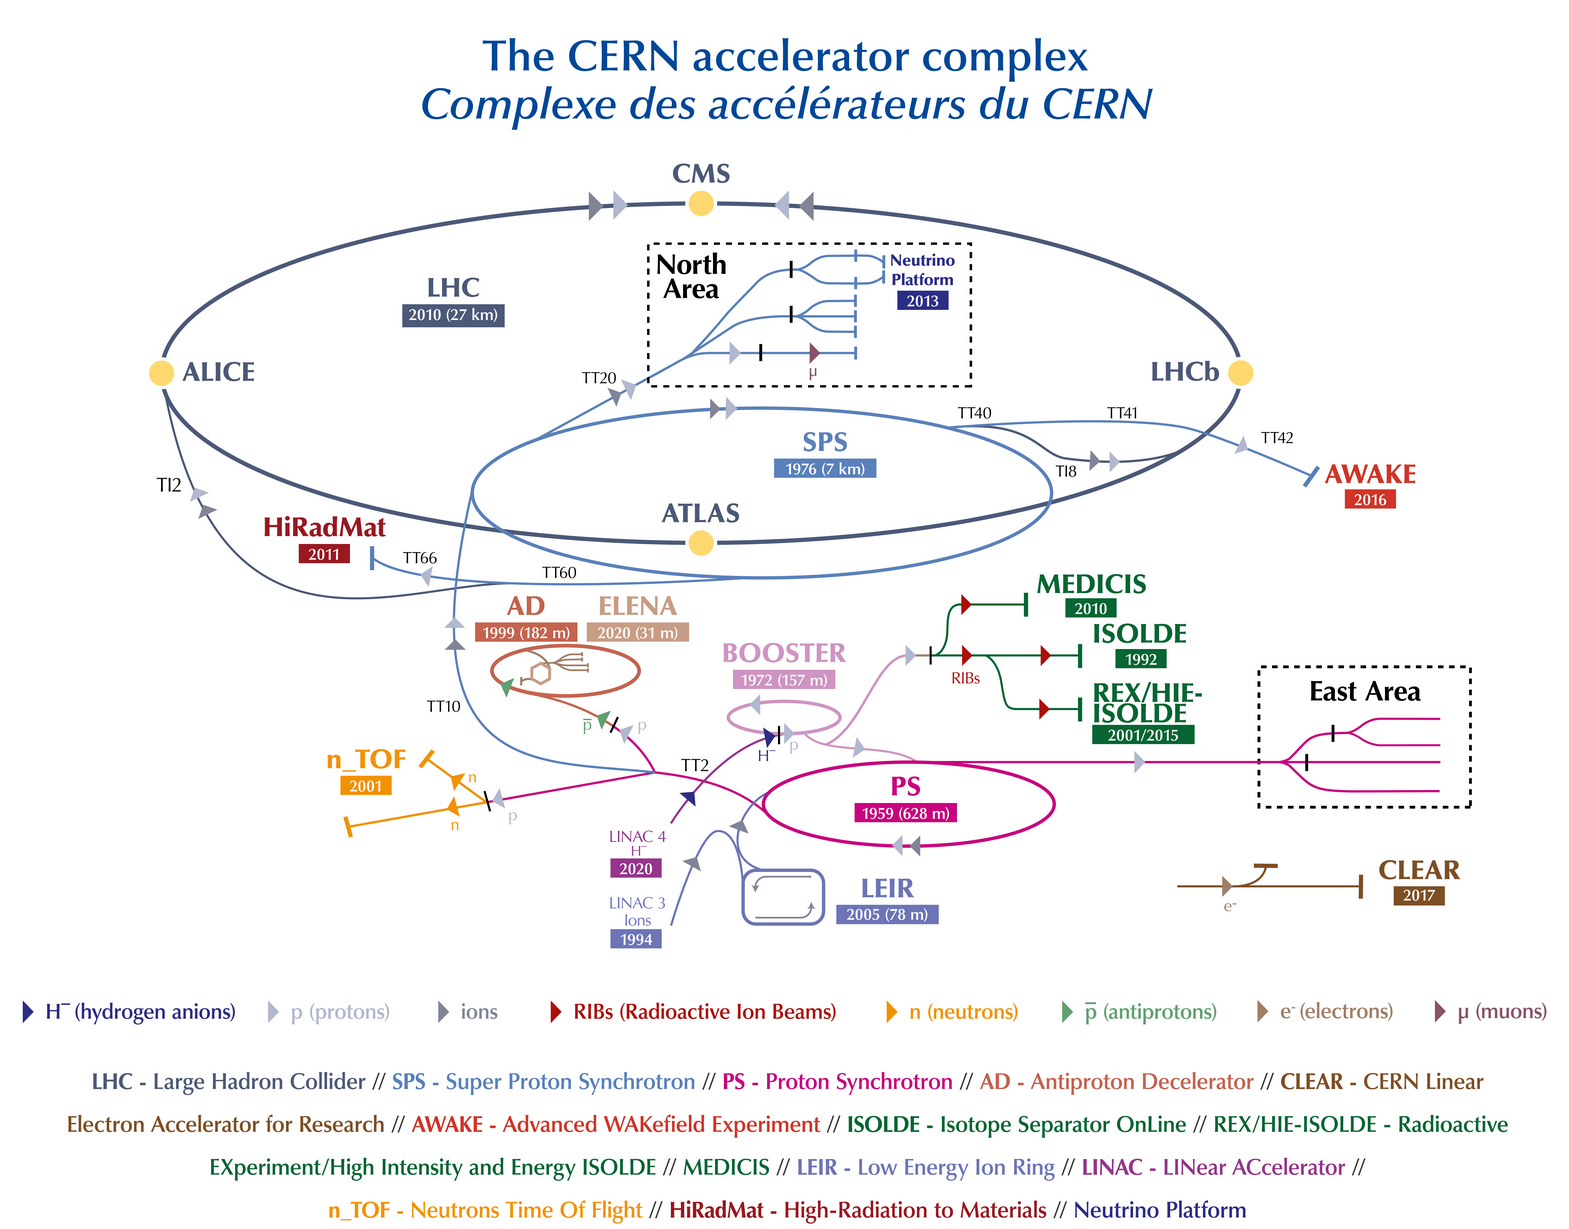
\includegraphics[width=0.99\textwidth]{Figures/cern_atlas/complex.png}
    \caption{The layout of the CERN accelerator complex as of 2022~\cite{CERNAC}.}
    \label{fig:cern_accelerator_complex}
\end{figure}

\subsection{Coordinate Systems}

In collider experiments, the typical coordinate system places the origin at the nominal IP, which, for hermetic detectors like ATLAS, Alice, and CMS, is at the centre of the detector.
The coordinate systems used by these experiments are right-handed, as shown in \Cref{fig:atlas_coordinate_system}, with the $z$-axis points along the beamline, the $y$-axis pointing upwards, and the $x$-axis pointing towards the centre of the LHC ring.
The transverse plane is defined as the plane perpendicular to the beam axis and is spanned by the $x$ and $y$ coordinates.

A polar representation is also often used, where the azimuthal angle $\phi$ is measured in the transverse plane from the $x$-axis, and the polar angle $\theta$ is measured from the $z$-axis.
The polar angle is frequently replaced with pseudorapidity $\eta$, defined as
\begin{equation}
    \eta = -\ln \left( \tan \left( \frac{\theta}{2} \right) \right).
\end{equation}
Differences in pseudorapidity are Lorentz invariant under boosts in the direction of the beamline, making it a useful quantity for describing the products of high-energy collisions.

Angular distances between objects are often measured in $\Delta R = \sqrt{(\Delta \eta)^2 + (\Delta \phi)^2}$, where $\Delta \eta$ and $\Delta \phi$ are the differences in pseudorapidity and azimuthal angle.
For collision products, a key observable is a transverse momentum $\pt=\sqrt{p_x^2 + p_y^2}$, where $p_x$ and $p_y$ are the components of the momentum in the transverse plane.

\begin{figure}
    \centering
    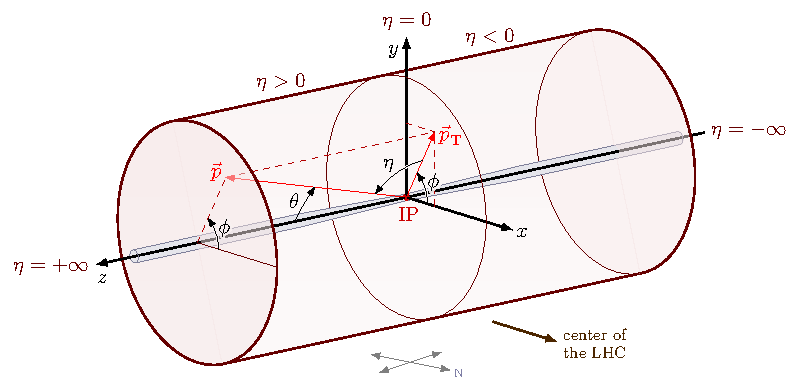
\includegraphics[width=0.6\textwidth]{Feynman/coordinate.pdf}
    \caption{The right-handed coordinate system used by the ATLAS experiment.}
    \label{fig:atlas_coordinate_system}
\end{figure}

\subsection{Cross-Section and Luminosity}

The cross-section, denoted by $\sigma$, indicates the likelihood of an interaction between two colliding particles.
Although calculating the cross-section involves quantum mechanical transition matrix elements and phase space integrals, it can be likened to the effective cross-sectional area of the particles participating in the interaction.

The total number of interactions $N$ depends on the cross-section of the process $\sigma$ and the integrated luminosity $L_{\text{int}}$ by the formula,
\begin{equation}
    N = \sigma L_{\text{int}} = \sigma \int \mathcal{L}(t) dt,
\end{equation}
where $\mathcal{L}(t)$ is the instantaneous luminosity.
This measures how tightly packed colliding particles are in a unit of space and time.
For two colliding beams with Gaussian densities, the instantaneous luminosity is given by
\begin{equation}
    \mathcal{L}(t) = \frac{N_1 N_2 f}{4 \pi \sigma_x \sigma_y} S(\theta_c),
\end{equation}
where $N_1$ and $N_2$ are the number of particles in each beam, $f$ is the frequency of bunch crossings, $\sigma_x$ and $\sigma_y$ are the root-mean-square beam widths in the $x$ and $y$ directions, and $S(\theta_c)$ is the geometric reduction factor due to the crossing angle $\theta_c$.
This last factor exists because the beams do not collide head-on, as this would result in multiple collision points, so they are crossed at a finite angle $\theta_c$.
This reduces the overlap of the beams when they pass through one another, reducing the effective luminosity.
For the $pp$ collisions at the LHC $S(\theta_c)$ is approximately $0.61$.
Even with this finite angle, long-range beam-beam interactions can still occur and must be accounted for.

The LHC was designed to deliver $\mathcal{L}(t) = 10^{34}~\unit{\centi\meter^{-2}\second^{-1}}$ at the IPs of ATLAS and CMS.
However, this has not been constant over the years, and each experiment independently measures the luminosity using well-understood processes.
The total integrated luminosity delivered by the LHC and recorded by ATLAS is shown in \Cref{fig:luminosity}.
The LHC's instantaneous luminosity has increased with each run and this is important as it boosts the production rate of all physical processes.
It particularly beneficial for measurements on rare events where the uncertainty is statistically limited.

\begin{figure}
    \centering
    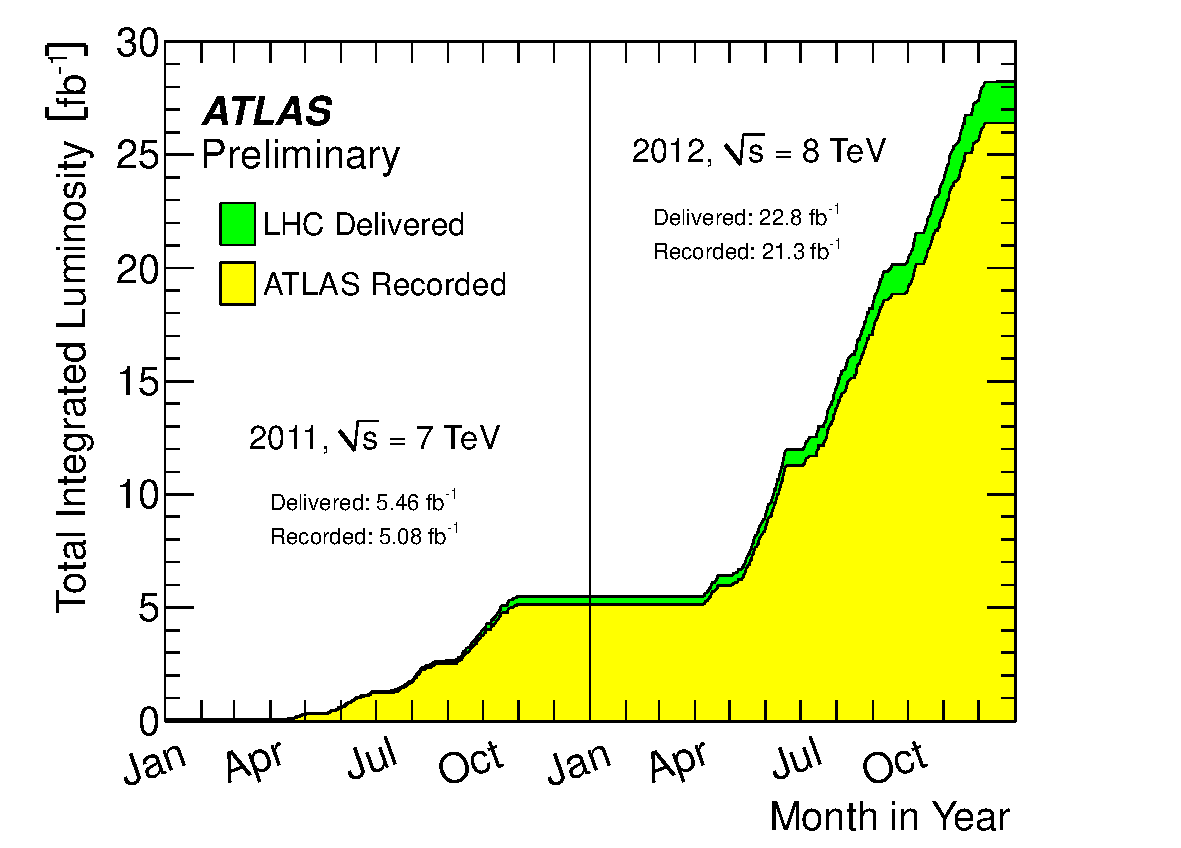
\includegraphics[width=0.32\textwidth]{Figures/cern_atlas/lumi1.pdf}
    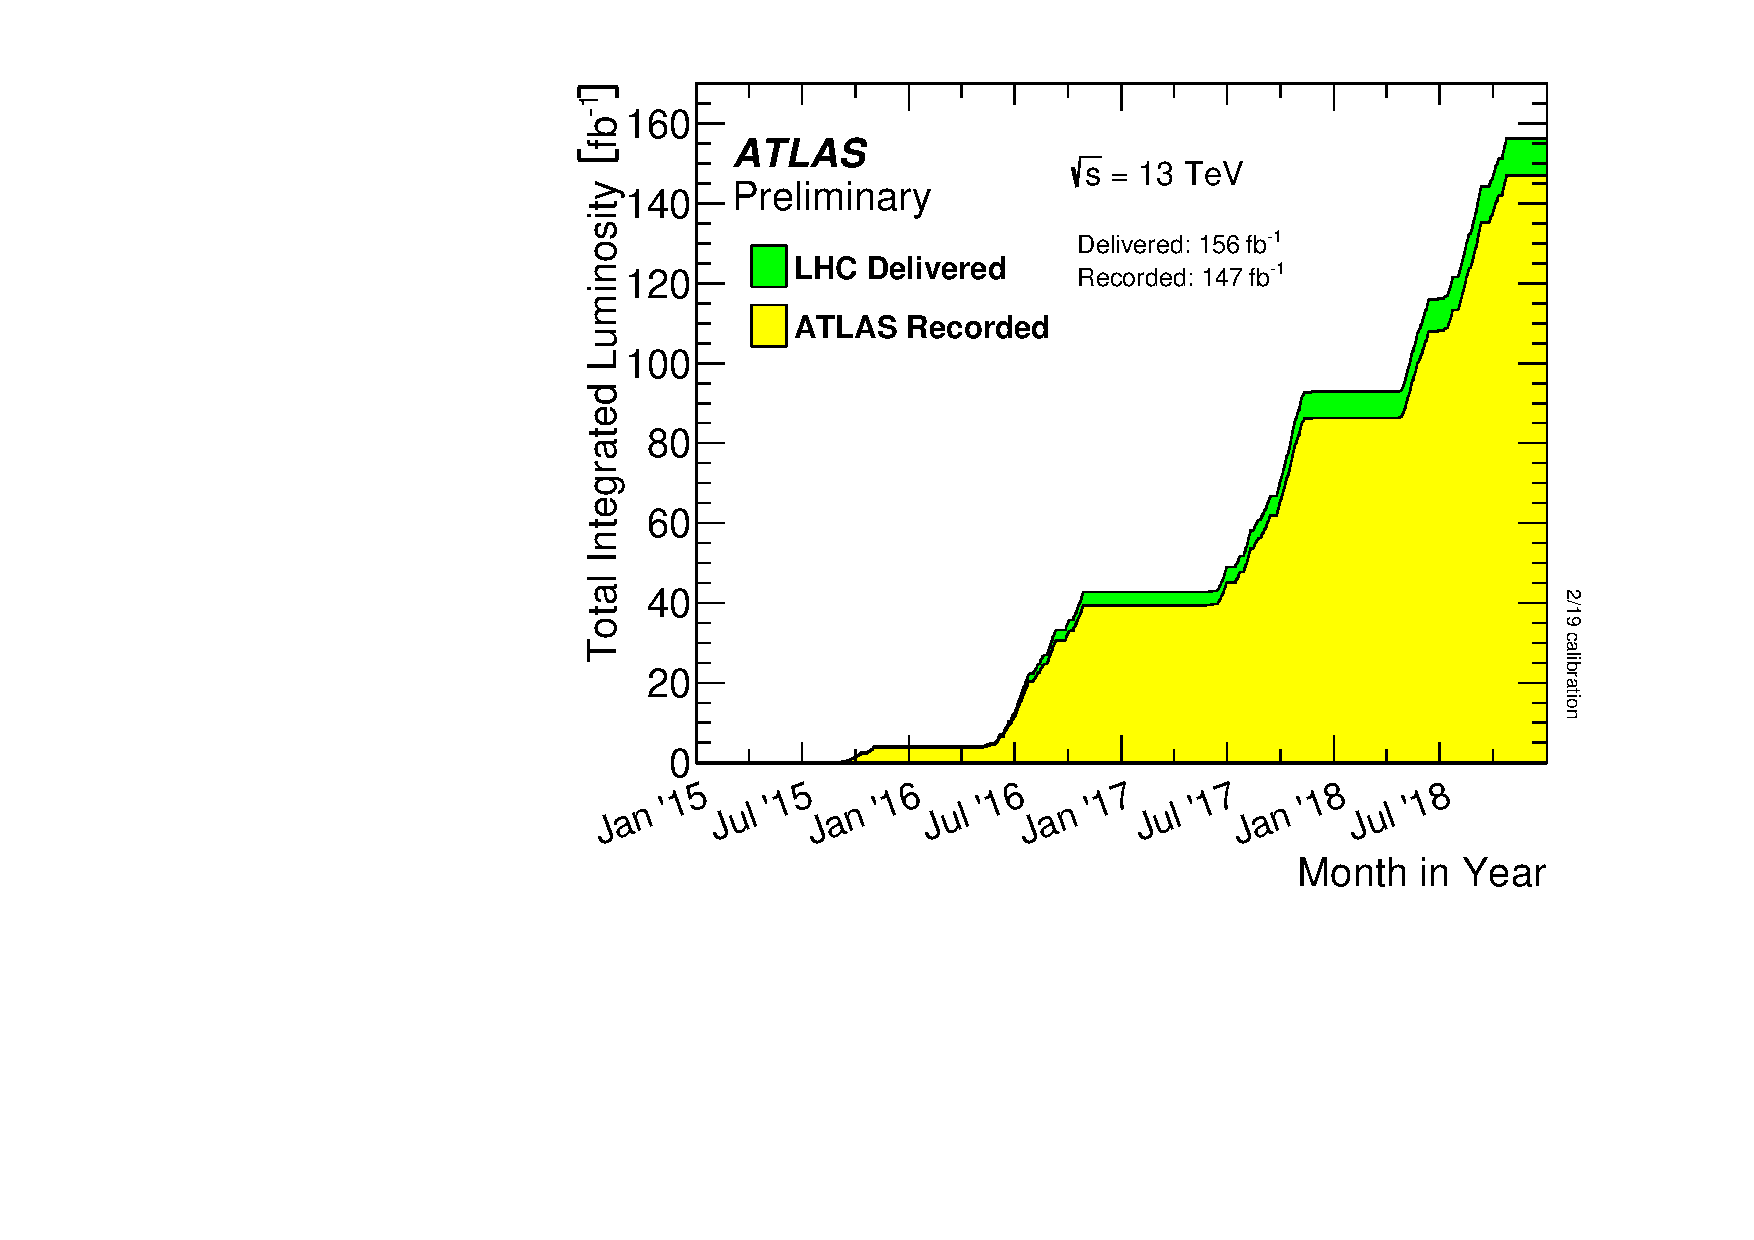
\includegraphics[width=0.32\textwidth]{Figures/cern_atlas/lumi2.pdf}
    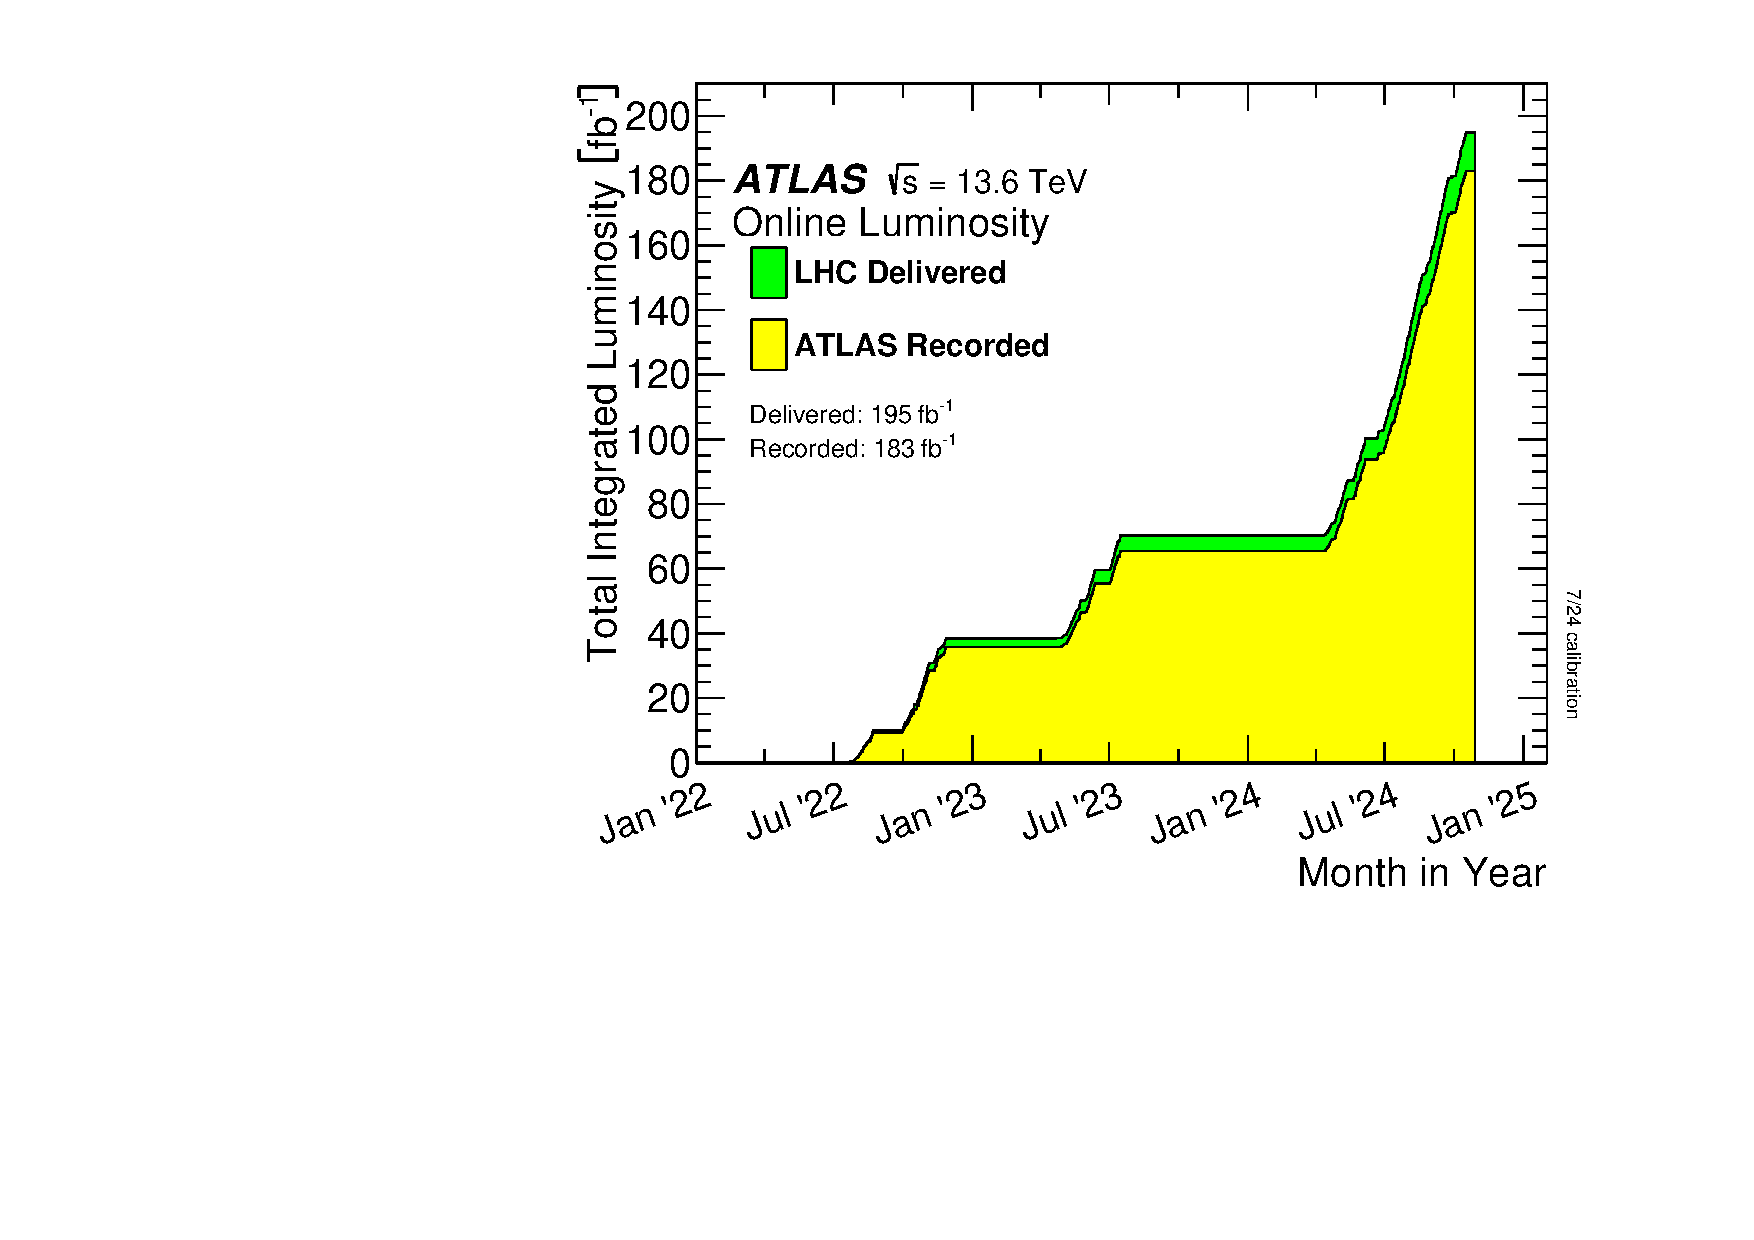
\includegraphics[width=0.32\textwidth]{Figures/cern_atlas/lumi3.pdf}
    \caption{The total integrated luminosity delivered by the LHC and recorded by the ATLAS experiment for Run 1 (left)~\cite{run1data}, Run 2 (middle)~\cite{run2data}, and Run 3 (right)~\cite{run3data}.}
    \label{fig:luminosity}
\end{figure}

\subsection{Pileup}

The increase in luminosity between Run 1 and Run 3 was in part achieved by raising the number of protons per bunch.
This in turn leads to more particle interactions per bunch crossing.
One of the undesirable effects of this is the large amount of overlapping signals in the detector which can degrade the resolution and efficiency of reconstruction algorithms.

Each bunch crossing in the collider generates a distinct event for analysis.
While the average number of interactions per crossing has increased with each LHC run, \Cref{fig:pileup} shows a wide distribution of interaction counts within each run.
Generally, only one of these interactions -- the hard scatter -- produces the high-energy particles captured by the detector and thus is of primary interest.
The remaining ``soft scatters'' are low-energy interactions that are known as in-time pileup.
Detector materials have a response and reset time, which can lead to residual signals from previous crossing being rerecorded, this is known as out-of-time pileup.
Filtering out signals from all pileup sources is crucial for accurate data analysis and poses a significant challenge as the LHC's luminosity increases.

\begin{figure}
    \centering
    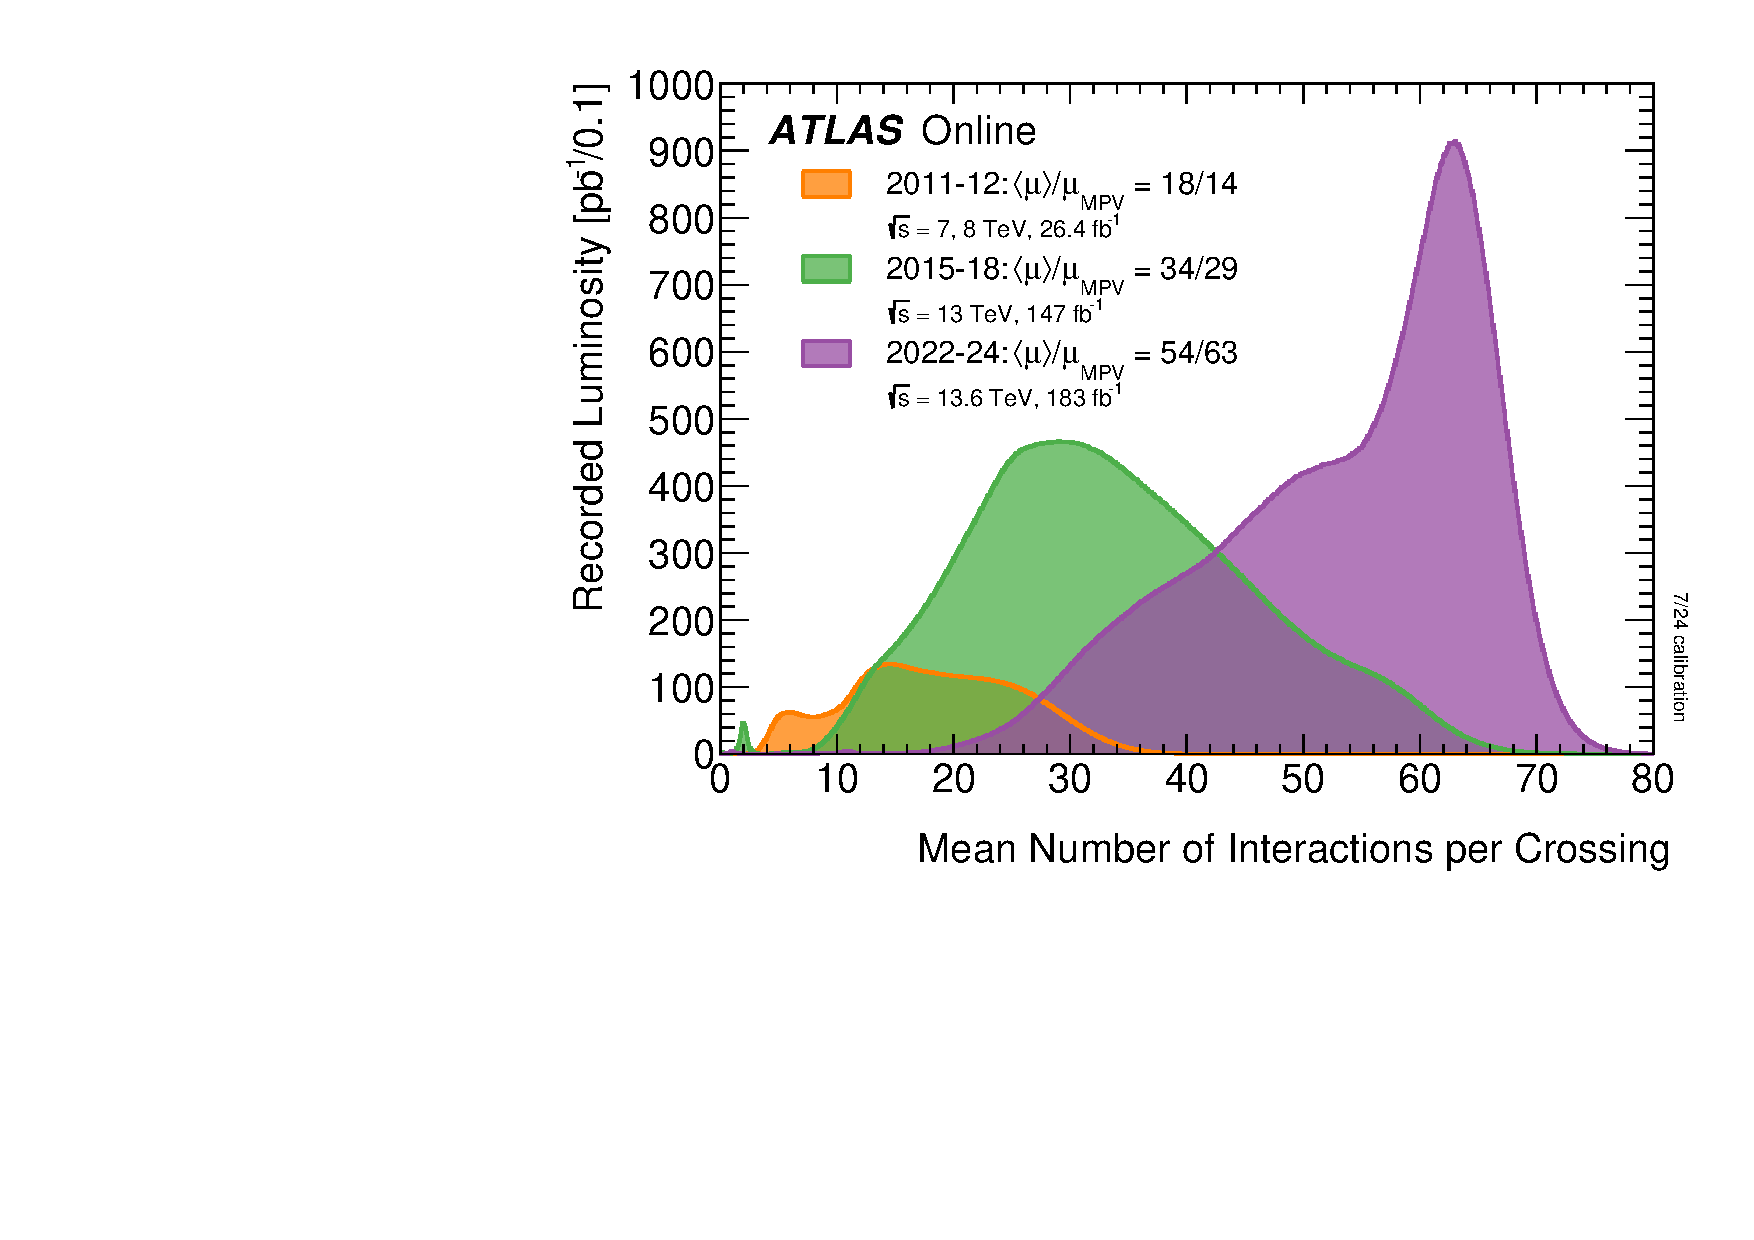
\includegraphics[width=0.6\textwidth]{Figures/cern_atlas/mu_run123.pdf}
    \caption{The distribution of the number of interactions per bunch crossing over the three LHC runs as measured by the ATLAS experiment~\cite{run3data}.}
    \label{fig:pileup}
\end{figure}

\subsection{LHC Runs}

The LHC operates on multi-year runs, the first beginning in 2010.
In between each run is a period of \textit{long-shutdown}, allowing for maintenance and upgrades to both the accelerator and the experiments.
The various run properties are shown in \Cref{tab:lhc_runs}.
Due to an electrical fault damaging many of the superconducting magnets in 2008, Run 1 was much delayed and operated at a reduced $\sqrt{s}=7~\TeV$ using a sparse bunch structure, only colliding at $20~\MHz$.
In 2012, the energy was increased to $\sqrt{s}=8~\TeV$.
The total delivered luminosity of the run was $28.4~\ifb$.
Run 2 spanned from 2015 to 2018, with an increased energy of $\sqrt{s}=13~\TeV$, a bunch crossing rate of $40~\MHz$, and a total integrated luminosity of $156~\ifb$.
Run 3 began in 2022 and is expected to continue until 2026 and has already surpassed Run 2 with $195~\ifb$ of data delivered~\cite{run3data}.

\begin{table}[h!]
    \centering
    \caption{Overview of the different LHC runs~\cite{LHCRun2,LHCRun3,run1data, run2data, run3data}. Values for Run 3 are preliminary as data is still being collected.}
    \label{tab:lhc_runs}
    \resizebox{\textwidth}{!}{
        \begin{tabular}{lcccccc}
            \toprule
                              & $\sqrt{s}~[\TeV]$ & $\mathcal{L}_\text{int}~[\ifb]$ & Protons per bunch     & Bunch spacing $[\ns]$ & \avemu \\
            \midrule
            Run 1 (2010-2011) & 7                 & 5.5                             & $1.45 \times 10^{11}$ & 50                    & 10     \\
            Run 1 (2012)      & 8                 & 22.8                            & $1.6 \times 10^{11}$  & 50                    & 21     \\
            Run 2 (2015-2028) & 13                & 156                             & $1.25 \times 10^{11}$ & 25                    & 34     \\
            Run 3 (2022-)     & 13.6              & 195                             & $1.8 \times 10^{11}$  & 25                    & 50     \\
            \bottomrule
        \end{tabular}
    }
\end{table}


% \section{The ATLAS Detector}

% \section{Event Reconstruction}
% \label{sec:event_reconstruction}

% \subsection{Tracks}

% The trajectory of a charged particle (track) is parameterized as a helix using five parameters:

% Impact parameter significances are calculated as:

% In flavor tagging, IP significances are lifetime signed:

% \begin{itemize}
%     \item $d_0$ and $z_0$: Transverse and longitudinal impact parameters (IP), specifying the closest approach of the track to the primary vertex.
%     \item $\phi$ and $\theta$: Azimuthal and polar angles.
%     \item $q/p$: Measured charge divided by the scalar 3-momentum.
%     \item $s(d_0) = \frac{d_0}{\sigma(d_0)}$
%     \item $s(z_0) = \frac{z_0}{\sigma(z_0)}$
%     \item Positive: Track crosses the jet axis in front of the primary vertex.
%     \item Negative: Track crosses the jet axis behind the primary vertex.
% \end{itemize}

% \subsection{Jets}

% For example, the differentiable cross-section of the ($2\rightarrow n+1$) process in \Cref{fig:quark_gluon} in the extreme soft and collinear limits factorizes into a $2 \rightarrow n$ process times a $1 \rightarrow 2$ split.
% In this extreme limit the probability for soft-colinear gluon emission is given by,
% \begin{equation}
%     \label{eq:gluon_emission}
%     d \mathcal{S} = \frac{2 \alpha_s C_F}{\pi} \frac{d \theta}{\sin\theta} \frac{dE}{E} \frac{d\phi}{2\pi},
% \end{equation}
% where $C_F = \sfrac{4}{3}$ is the color factor for the quarks, $\theta$ is the angle of the emitted gluon with respect to the quark, $E$ is the energy of the emitted gluon, and $\phi$ is the azimuthal angle.

% \subsubsection{Particle Flow}
% \label{sec:particle_flow}

% \subsubsection{Fat Jets}
% \label{sec:fat_jets}

% At the LHC, quarks can be produced in the decays of particles such as $W/Z$~bosons, or top quarks through their decay into a $W$~boson and a $b$-quark.
% For most energy scales, the two or three quarks from these decays produce jets that can be individually resolved in the detector.
% However, as the momenta of the intermediate particles increase, the decay products themselves start to collimate, resulting in a single large-radius or \textit{fat} jet in the detector; this is the so-called boosted regime.
% These objects are colloquially referred to as \textit{fat jets}.
% The vast majority of jets, however, are initiated by partons, which are not the decay products of other massive particles (QCD background).
% https://tikz.net/jet_top/

% \subsection{Jet substructure}
% \label{sec:jet_substructure}
% Properties relating to the distribution of constituents within a jet are known as the substructure of a jet, which can be used to identify the original seed particle~\cite{Kogler:2018hem}.
% This is particularly interesting in the boosted regime, where several partons from the decay of another elementary particle have overlapping showers.
% % In boosted topologies it is of particular interest to identify whether a jet is from hadronic decays of a resonant particle or otherwise.
% % Therefore, accurate modelling of jet substructure is of importance in many measurements and searches at the LHC.
% % Many high level features are defined based on physics principles and are calculated from the constituents in a jet.

% One commonly used set of observables to describe jet substructure is its \emph{N-subjettiness}~\cite{Thaler_2011}, denoted by ${\tau_N}$.
% These are useful in identifying jets originating from processes with $N$ prongs as a result of the decay of the initial particle.
% A jet originating from a gluon is likely to have a 1-prong substructure, whereas a $W/Z$~boson decay is likely to produce a 2-prong jet, and a jet originating from the all-hadronic decay of a top quark will tend to be 3-prong.
% Other commonly used observables relate to the energy correlation functions of a jet and their ratios, such as $\Dtwo$~\cite{Larkoski_2013,Larkoski_2014}.%
% \footnote{$\Dtwo$ is defined as the ratio of the three-point and cubed two-point energy correlation functions.}
% A new set of features which have been found to be sensitive to the underlying substructure of different jet types are the Energy Flow Polynomials~(EFPs)~\cite{Komiske_2018}.

% Furthermore, when a seed particle decays, the observed opening angle of the decay products is strongly dependent on its mass and momentum.
% In jets, this means that the distribution of constituent properties is strongly correlated to the overall invariant mass and transverse momentum \pt.

% Classification approaches applying cuts on the substructure features, as well as machine learning algorithms trained using such features have been successfully employed in the ATLAS and CMS collaborations to distinguish jets originating from $W$~bosons ($W$-jets), top quarks (top jets), gluons, and light quarks~\cite{ATLAS:2018wis,CMS:2020poo}.
% In recent years, more sophisticated classification algorithms have been trained on the constituents themselves, either represented as ordered vectors~\cite{pearkes2017jet,ATLAS:2018wis,CMS:2020poo,Butter_2018}, images~\cite{de_Oliveira_2016,Kasieczka_2017,Macaluso_2018}, or point clouds~\cite{ParticleNet,Komiske:2018cqr,Moreno:2019bmu,Dreyer:2020brq,Dolan:2020qkr,Mikuni:2021pou,Shimmin:2021pkm,Gong:2022lye,Qu:2022mxj} (see Ref.~\cite{TopLandscape} for a review).

% These approaches are very sensitive to the substructure of jets originating from different particles.
% As such, when using fast surrogate models it is crucial that they accurately capture the distribution of the constituents within a jet and their correlations to the mass and \pt.

% \section{Event Simulation}

% \section{Flavour Tagging}
% \label{sec:flavour_tagging}

% A diagram of the GN1 model is shown in \Cref{fig:gn1}.

% \begin{figure}
%     \centering
%     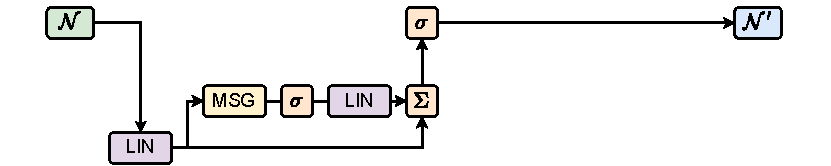
\includegraphics[width=0.99\textwidth]{figures/atlas/gn1.png}
%     \caption{Schematic diagram of the GN1 model from Ref.~\cite{GN1}.}
%     \label{fig:gn1}
% \end{figure}
